\chapter{Background}%
\label{cha:background}

This chapter will give some background about how Scratch works and why testing Scratch programs is a difficult task.
It will also highlight some previous approaches towards automated assessment of Scratch programs.

\section{Scratch}%
\label{sec:scratch}

Scratch~\cite{scratch} is a programming language developed by the MIT Media Lab.
Its main goal is to offer an intuitive language suited for programming novices and children.
Scratch implements a block-based code system, which eliminates the possibility of syntax errors.
It also allows users to easily integrate graphics and audio into their programs.
Code is run inside a special Scratch virtual machine.
Therefore, Scratch is exclusively developed and run through Scratch's web interface, which can be seen in Figure~\ref{fig:scratch_gui}.
\parspace

\begin{figure}[htpb]
    \centering
    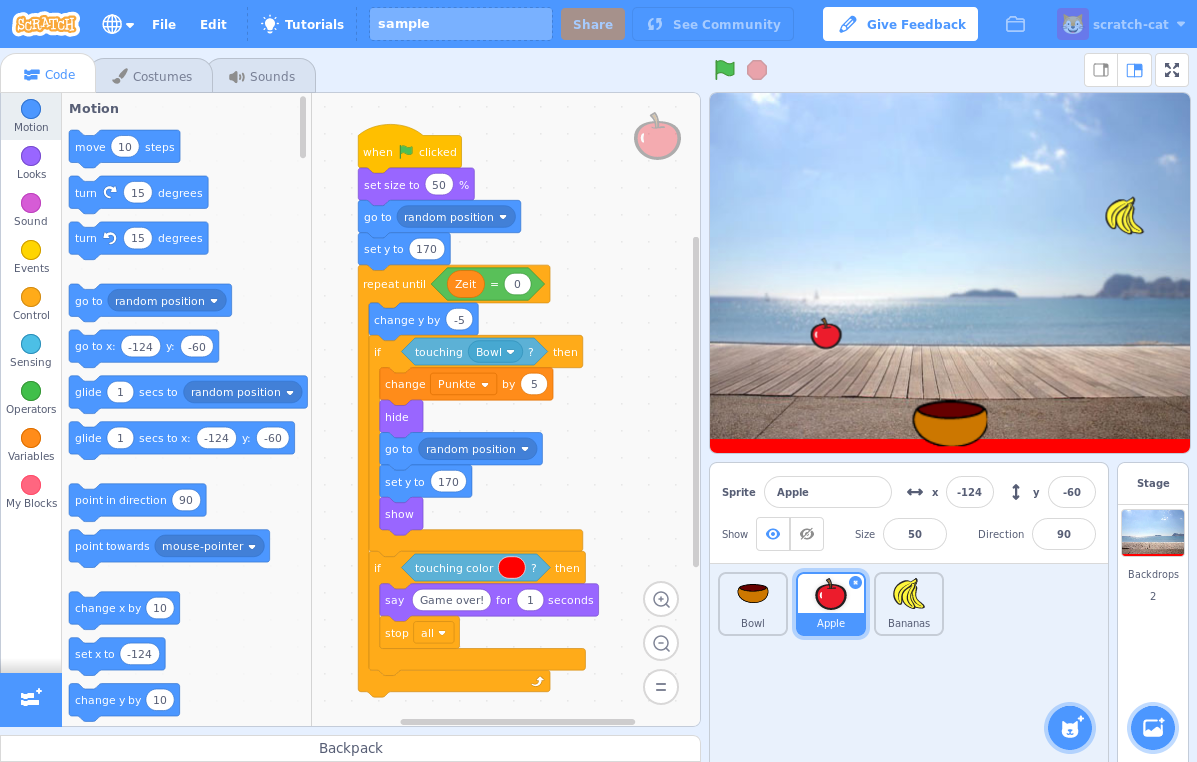
\includegraphics[width=0.75\textwidth]{scratch-gui}
    \caption{Scratch 3.0's web interface}
    \label{fig:scratch_gui}
\end{figure}

\textbf{Code.}
Programming in Scratch is done by sticking together a structure of pre-defined blocks, which are equivalent to statements and control
structures in traditional programming languages.
Multiple blocks are combined together with a \textit{hat} to make up a \textit{script}, as can be seen in Figure~\ref{fig:scratch_code}.
Scripts are called through a type of event, which is defined by their hat.
There are a variety of different events in Scratch.
The main event is the \textit{green flag} event, the entry point of the program.
This event is emitted when the user starts the program by pressing the green flag button.
The program then starts by executing all scripts that are equipped with a ''when green flag is pressed'' hat.
Other events include key presses on the keyboard, clicks on a specific sprite, and events sent from different scripts.
Active scripts effectively run in parallel until the end of each script is reached or until the script is stopped by itself or another script.
\parspace

\begin{figure}[htpb]
    \centering
    \scalebox{.95}{
        \begin{tikzpicture}
            \node[anchor=south west,inner sep=0] at (0, 0) {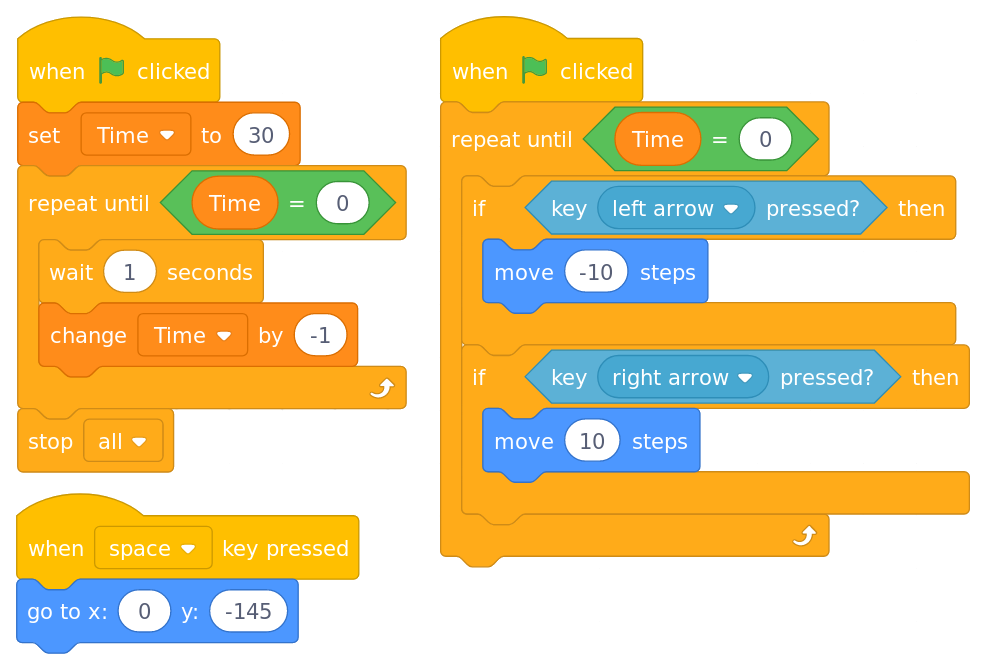
\includegraphics[width=0.6\textwidth]{scratch-code}};
            \draw[red, ultra thick, rounded corners]  (0, 5.27) rectangle (2.20, 6.10);
            \draw[blue, ultra thick, rounded corners] (0, 1.65) rectangle (3.90, 5.10);
            \node[red, font=\large, anchor=north east]   at (0, 6.00) {\texttt{Hat}};
            \node[blue, font=\large, anchor=north east]  at (0, 5.00) {\texttt{Code}};
        \end{tikzpicture}
    }
    \caption{Scratch scripts}
    \label{fig:scratch_code}
\end{figure}

\textbf{Input and output.}
Scratch programs create interactive two-dimensional animations through a number of visual objects (the \textit{sprites}) on a background (the \textit{stage}).
The program manipulates sprites' appearance, position, size, rotation, visual effects and sounds.
Furthermore, sprites can display messages and ask the user to type answers into a text box through \texttt{say} and \texttt{ask} blocks.
Variables can also be displayed on screen.
Programs can react to user input like keyboard key presses, mouse clicks or mouse cursor movement.
Scratch's visual output is rendered in a constant frequency of 30 times per second.
We will call the rendered pictures \textit{frames}.
\parspace

\textbf{Sprite and variables.}
Each sprite contains its own scripts and variables.
These variables, as well as the sprite itself can only be manipulated by the sprite's own scripts.
The only exception to this rule is the stage, whose variables are global.
Sprites can communicate with each other through a messaging system and through the stage's variables.
By \textit{cloning} sprites, the program can create multiple instances of a sprite, which behave alike.
The cloned sprites then also share the original sprite's variables.
\parspace

\textbf{Program execution.}
Scratch executes part of the program in a fixed frequency of 30 times per second.
We will call the program execution, that is done 30 times per second, a \textit{step}.
During the step, Scratch executes the program until either a certain time limit is reached,
a sprite changes its position or appearance, or all scripts are done (and the program finished), whichever happens first.
Then, a new frame is rendered.
The program is executed by running its's threads, which each run an instance of an active script, sequentially.
Each of the threads is executed until either the script's end is reached,
a loop iteration has been executed, or the thread yields (e.g. when a \texttt{wait} block is used).
Figure~\ref{fig:scratch_step_procedure} illustrates this procedure.
\parspace

\begin{figure}[htpb]
    \centering
    \tikzset{>=latex,
             arrow/.style={draw, -{Latex[length=1.5mm, width=1.5mm]}},
          bigarrow/.style={draw, -{Latex[length=2.5mm, width=2.5mm]}},
               num/.style={draw, circle, inner sep=0.6mm, text centered}}

    \begin{tikzpicture}[scale=0.7, every node/.style={scale=0.7}]
        \node[anchor=north west,inner sep=0] at (0, 0) {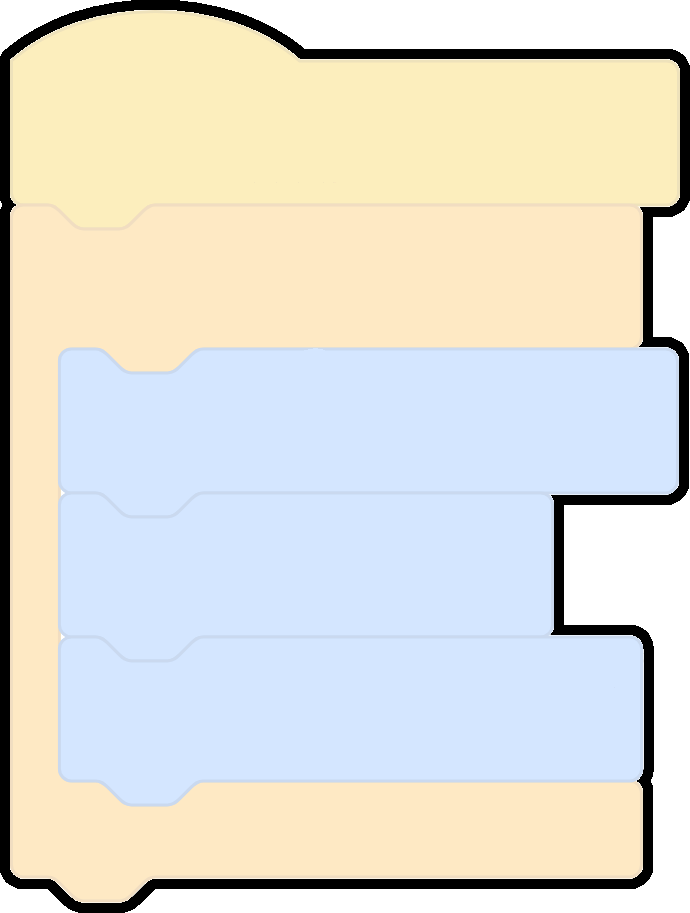
\includegraphics[width=0.20\textwidth]{scratch-script-scheme}};
        \node[anchor=north west,inner sep=0] at (4, 0) {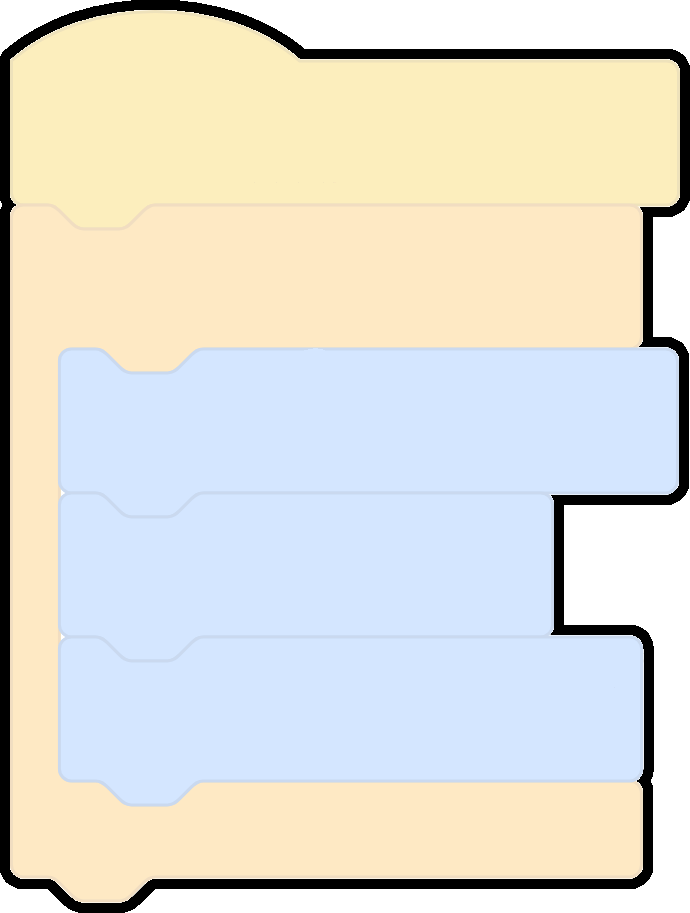
\includegraphics[width=0.20\textwidth]{scratch-script-scheme}};
        \node[anchor=north west,inner sep=0] at (8, 0) {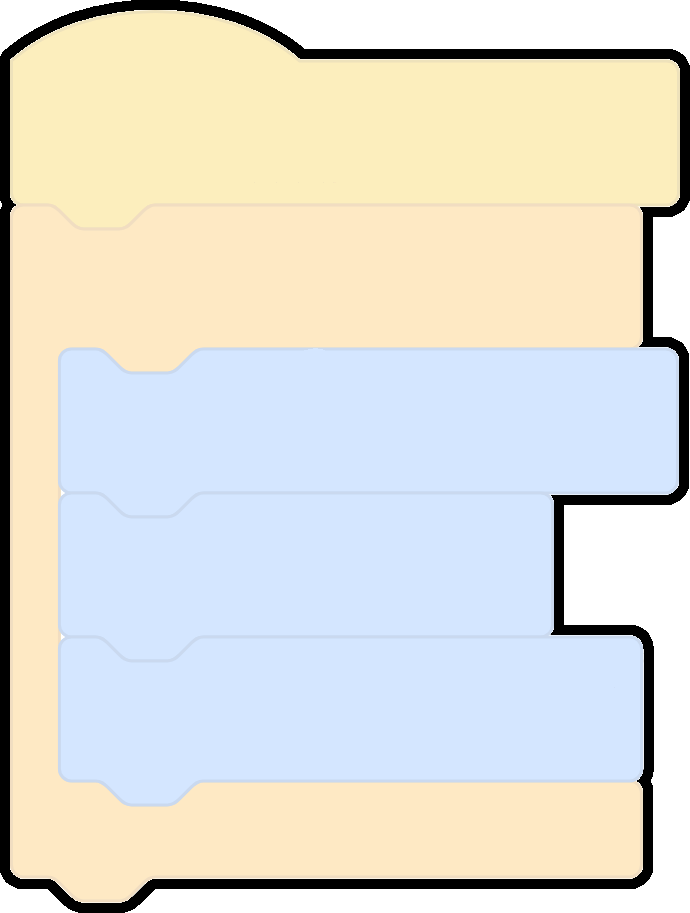
\includegraphics[width=0.20\textwidth]{scratch-script-scheme}};

        \draw[dashed, rounded corners]  (-1.85, 0.5) rectangle (11.5, -4.5);

        \node[]  at (1.5, -0.60) {Thread \texttt{\#}1};
        \node[]  at (5.5, -0.60) {Thread \texttt{\#}2};
        \node[]  at (9.5, -0.60) {Thread \texttt{\#}n};

        \node[num] at (-1, -2.35) {\large 1};

        \draw[thick, arrow] (2.75, -2.45) -- (3.8, -2.45);
        \draw[thick, arrow, dashed] (6.75, -2.45) -- (7.8, -2.45);

        \draw[thick, arrow, rounded corners]
               ( 0.5, -1.25)
            -- ( 0.5, -3.5)
            -- (-0.5, -3.5)
            -- (-0.5, -1.25)
            -- ( 0,   -1.25);

        \draw[thick, bigarrow, rounded corners]
               (11.5,  -2)
            -- (12.5,  -2)
            -- (12.5,  -5.5)
            -- (-2.85, -5.5)
            -- (-2.85, -2)
            -- (-1.85, -2);

        \node[num] at (-3.4, -3.75) {\large 2};

        \node at (3, -8.8) {
            \begin{varwidth}{\linewidth}
                \large
                \begin{enumerate}[nolistsep, noitemsep]
                    \item[(1)] Execute until ...
                        \begin{itemize}[nolistsep, noitemsep]
                            \item[...] the end of script is reached or
                            \item[...] one loop iteration has been executed or
                            \item[...] the script yields
                        \end{itemize}
                    \item[(2)] Loop until ...
                        \begin{itemize}[nolistsep, noitemsep]
                            \item[...] a certain time limit is reached or
                            \item[...] a sprite's position or appearance changes or
                            \item[...] all scripts are done
                        \end{itemize}
                \end{enumerate}
            \end{varwidth}
        };
    \end{tikzpicture}

    \caption{Scratch step procedure}
    \label{fig:scratch_step_procedure}
\end{figure}

\section{Previous Testing Approaches}%
\label{sec:previous_testing_approaches}

Although automated assessment of Scratch programs is still an open problem,
at least two other projects have tackled this task through different approaches.
\parspace

\textbf{Hairball.}
Boe et al. developed Hairball~\cite{hairball} to perform static analysis on Scratch programs.
Hairball is implemented as a standalone Python program.
It allows users to load a saved Scratch project file and analyze it by iterating through its blocks.
An example application of this program is the web-based assessment tool called Dr.\ Scratch~\cite{drscratch} by Moreno-Le\'on et al.,
which uses Hairball to measure the complexity of Scratch programs in various categories and scores them accordingly.
Though Hairball is very useful for analyzing programs statically, testing the functionality of a program with it would be very difficult.
In order to do this, a dynamic testing approach is more suitable, because tests can simply observe to program's behaviour instead of having to deduct it from the programs source code.
\parspace

\textbf{ITCH.}
ITCH (Individual Testing of Computer Homework for Scratch Assignments)~\cite{itch} by David E. Johnson is another Scratch assessment tool.
Like Hairball, it is also implemented in Python.
But it follows an entirely different approach.
ITCH performs functional testing on Scratch programs, which have their functionality reduced to simple textual input and output operations.
Scratch supports these operations through \texttt{ask} and \texttt{say} blocks.
In order to automate the IO, ITCH replaces these blocks with structures, that give the program configured input text and record the resulting output.
ITCH then executes the program, saves it, which also saves the current state of the variables, and analyzes the saved project file to generate a test report.
This allows simple input-output-testing for Scratch, which is useful for testing the correctness of an implemented algorithm.
But ITCH has a major drawback: Reducing Scratch programs to textual IO means that only a small subset of Scratch's functionality is available to the programs under test.
Sprite manipulation and such cannot be tested with ITCH.
If the only reason to adopt Scratch is its block-based code system, there exist other block-based programming environments, that serve as a front-end to more common programming languages, which can be tested more easily.
An example for this is BlockPy~\cite{blockpy}, which translates its block-based code into Python.

\section{Challenges of Testing Scratch Programs}
\label{sec:challenges_of_testing_scratch_programs}

Functional testing for Scratch is not a straightforward task.
There exist multiple challenges, that have to be overcome in order to test Scratch programs.
This section will go over some of these challenges and explain each of them.
\parspace

\textbf{Scratch's code system.}
Scratch does not have a traditional mechanism to structure code into methods, that return values.
Unit tests often call methods with some input and check the returned value, but this is not possible in Scratch.
Additionally, scripts run in parallel and may depend on one another.
This makes it hard to test a part of the program in isolation from the rest of the program.
One could circumvent this problem by restricting the tested programs, like ITCH~\cite{itch} does it,
but that defeats the purpose of using Scratch as a language.
\parspace

\textbf{GUI input and output.}
Scratch is entirely run inside a graphical user interface and lacks traditional IO mechanisms.
Its output consists of visual animations and audio, which are difficult to analyze automatically.
Likewise, Scratch's input, which mainly consists of keyboard and mouse input, can make interacting with the program in an automated way problematic.
\parspace

\textbf{Randomness.}
Scratch provides blocks to incorporate randomness into programs.
Non-determinism is problematic for testing in general and not just for Scratch,
but Scratch programs tend to frequently make use of randomness,
since the programs implemented in Scratch are often of game-like nature.
\parspace

\textbf{Missing Initialization.}
Scratch programs don't start with a fixed configuration of sprites and variables.
When the program is loaded, sprite attributes and variable values are restored from the project file,
but subsequent program executions after the first one start with the configuration in which the last execution left the sprites and variables in.
Scratch programs can deal with this by doing initialization in the beginning, but many implementations don't.
\parspace

\textbf{Fuzziness of properties.}
Scratch programs don't usually deal with exact values,
since small differences in sprite properties are generally indistinguishable in the program's graphical output.
This can make testing more difficult, since assertions may have to take small deviations into consideration.
Scratch itself also makes dealing with exact values unattractive.
In the Scratch GUI, sprites can initially be positioned on the stage via drag and drop,
and instead of comparing exact positions, Scratch offers built in blocks to directly check for sprite collisions.
\parspace

\textbf{Tracking of properties.}
In order to test sprite movements and animations, sprite attributes need to be tracked over a period of time.
Hence, sprite attributes need to be accessible periodically during the program execution.
\parspace
